\section{Część sprzętowa}

\begin{figure}[t]
    \begin{center}
       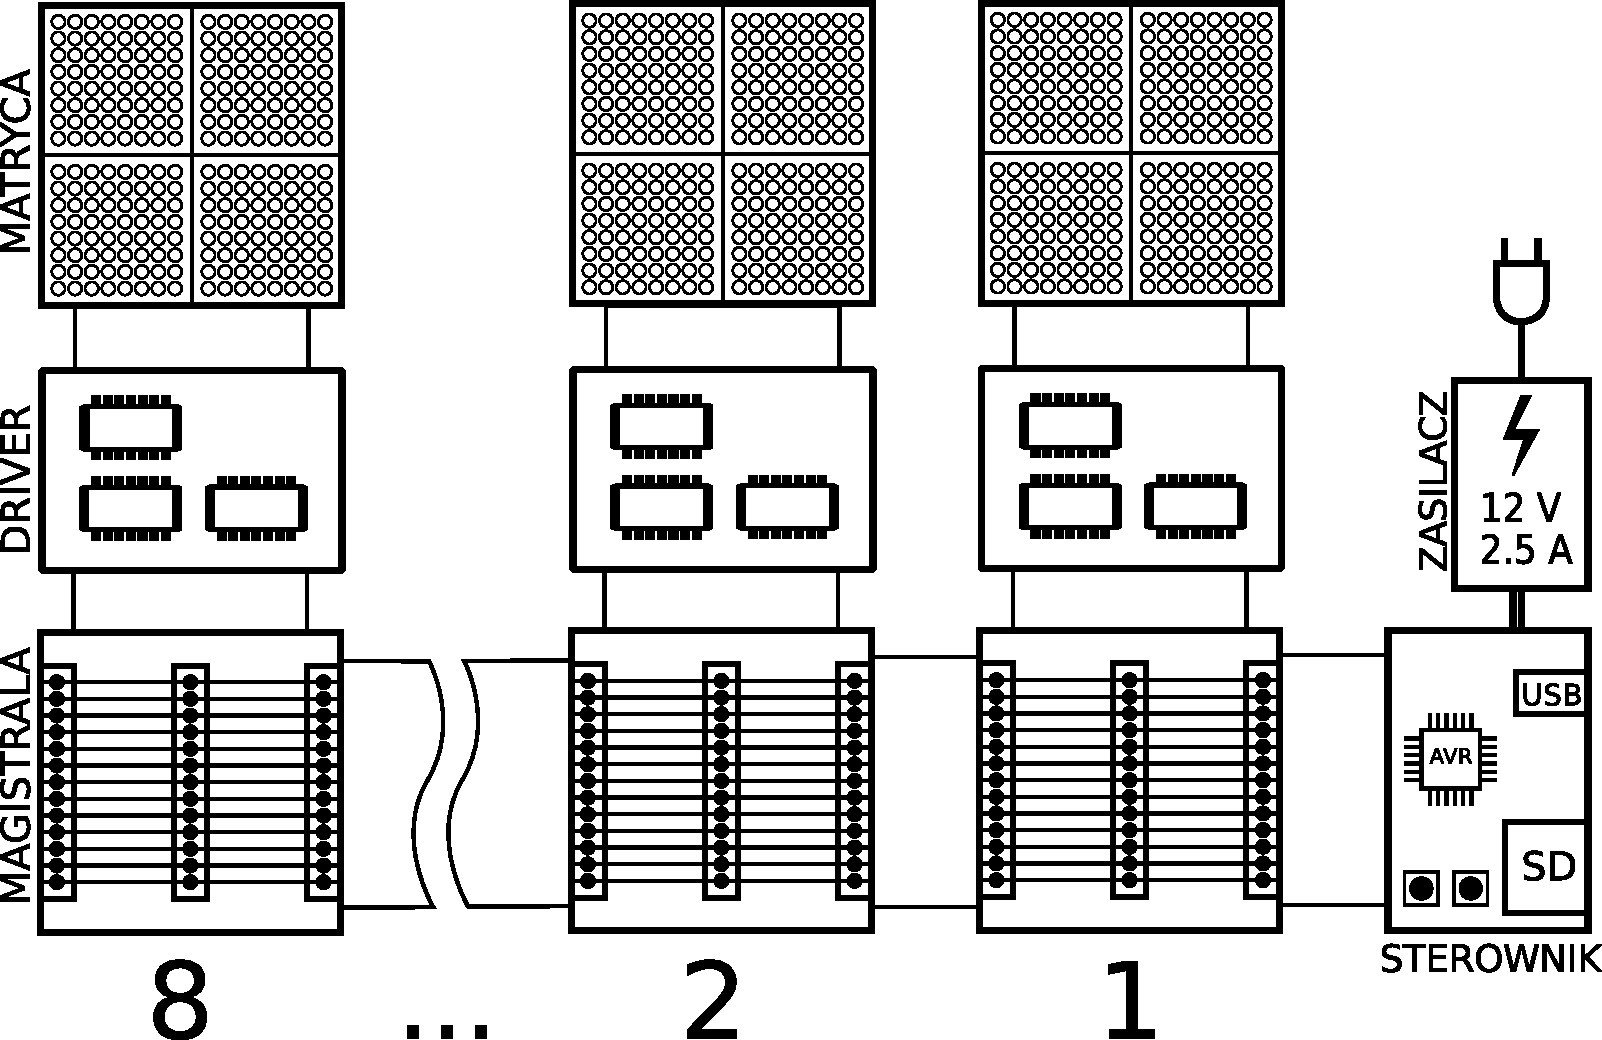
\includegraphics[width=\textwidth]{figures/blokowy.pdf}
    \end{center}

    \caption{Schemat blokowy urządzenia.}
    \label{schemat-blokowy}
\end{figure}

Urządzenie ma budowę modułową, co pozwala na różnorodną konfigurację i~dostosowanie go do istniejących potrzeb. Każdy moduł posiada swą własną płytkę drukowaną.  Schemat blokowy widoczny na rysunku \ref{schemat-blokowy}. Wyróżnić można na nim następujące elementy:
\begin{itemize}
	\item \textbf{matryca} --- w~tablicy zainstalowano osiem takich modułów, co daje powierzchnię o~wymiarach $128 \times 16$ pikseli,
	\item \textbf{driver} --- osiem sztuk,
	\item \textbf{magistrala} --- rozprowadza sygnały sterujące i~zasilanie między drajwerami, osiem sztuk,
	\item \textbf{sterownik} --- generuje sygnały sterujące dla wyświetlaczy,
	\item \textbf{zasilacz sieciowy 12~V} --- o~wydajności $2.5$ A.~Przy aktywnych wszystkich pikselach prąd pobierany przez urządzenie sięga $2.3$ A.
\end{itemize}
Sterownik jest dziełem autorów pracy. Pozostałe moduły zostały dostarczone przez promotora lub też wykorzystano elementy fabryczne. Wszystkie moduły zostały dokładnie omówione poniżej.


\subsection{Opis dostarczonych modułów}

Moduły matrycy, drajwera i~magistrali zostały dostarczone przez promotora jako dane wejściowe pracy inżynierskiej.

\textbf{Moduł matrycy} grupuje cztery wyświetlacze matrycowe LED typu JZM23882ASR\-GW o~rozmiarze $ 8 \times 8 $ pikseli w~jeden o~wynikowym rozmiarze $16 \times 16$ pikseli. Wykonany został jako dwustronna płytka drukowana z~metalizacją otworów o~rozmiarach $136 \times 133$ mm. Nie zawiera elementów elektronicznych z~wyjątkiem wyżej wymienionych matryc LED.~Moduł łączy się z~drajwerem przez dwa szesnastopinowe wtyki goldpin. Jeden wtyk zajmują wyprowadzenia anod, drugi --- katod. Widok ogólny modułu przedstawia rysunek \ref{zdj-matryca}.

\begin{figure}[t]
    \begin{center}
       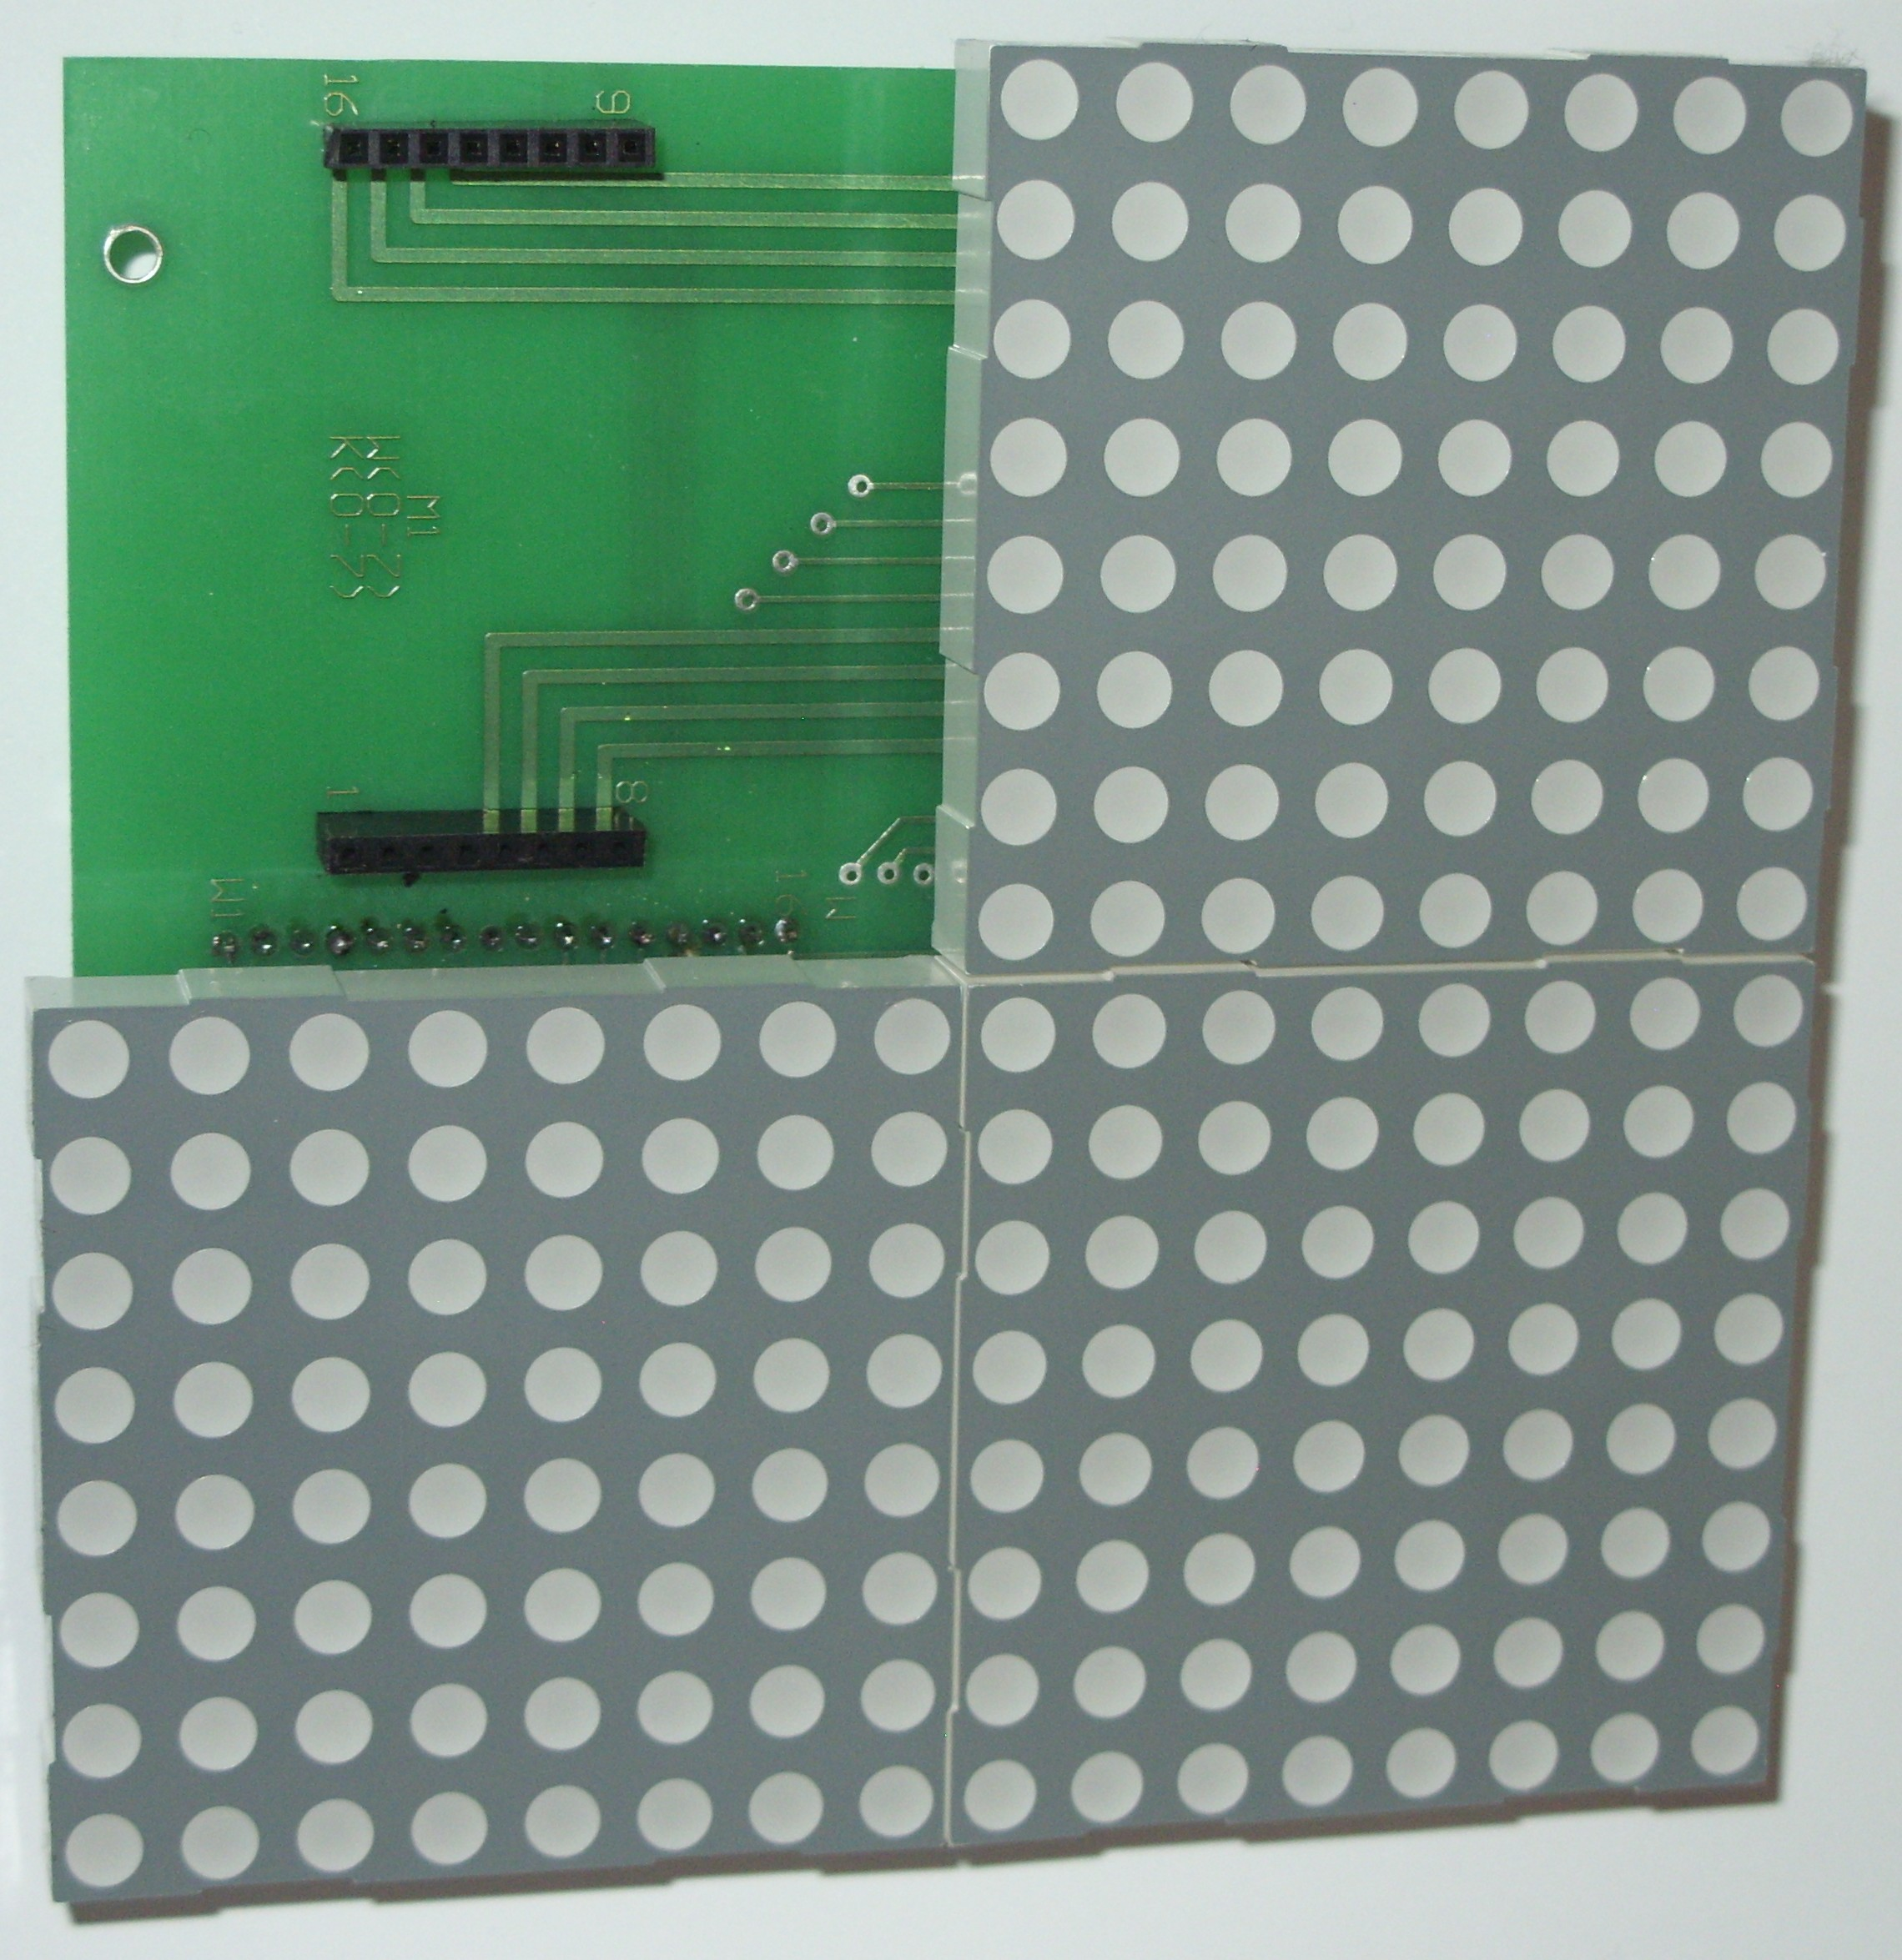
\includegraphics[width=0.8\textwidth]{figures/zdj-matryca.jpg}
    \end{center}

    \caption{Zdjęcie modułu matrycy. Widoczne trzy z czterech wyświetlaczy.}
    \label{zdj-matryca}
\end{figure}

\textbf{Moduł drajwera} odpowiada za odpowiednie sterowanie pojedynczym modułem matrycy. Schemat ideowy widoczny jest na rysunku \ref{zdj-driver}. Jednostronna płytka drukowana o~wymiarach $111 \times 32$ mm z~jednej strony łączy się z~magistralą 40-pinową wtyczką goldpin; z~płytką matrycy połączona jest dwoma 16-pinowymi gniazdami goldpin. 

\begin{figure}[t]
    \begin{center}
       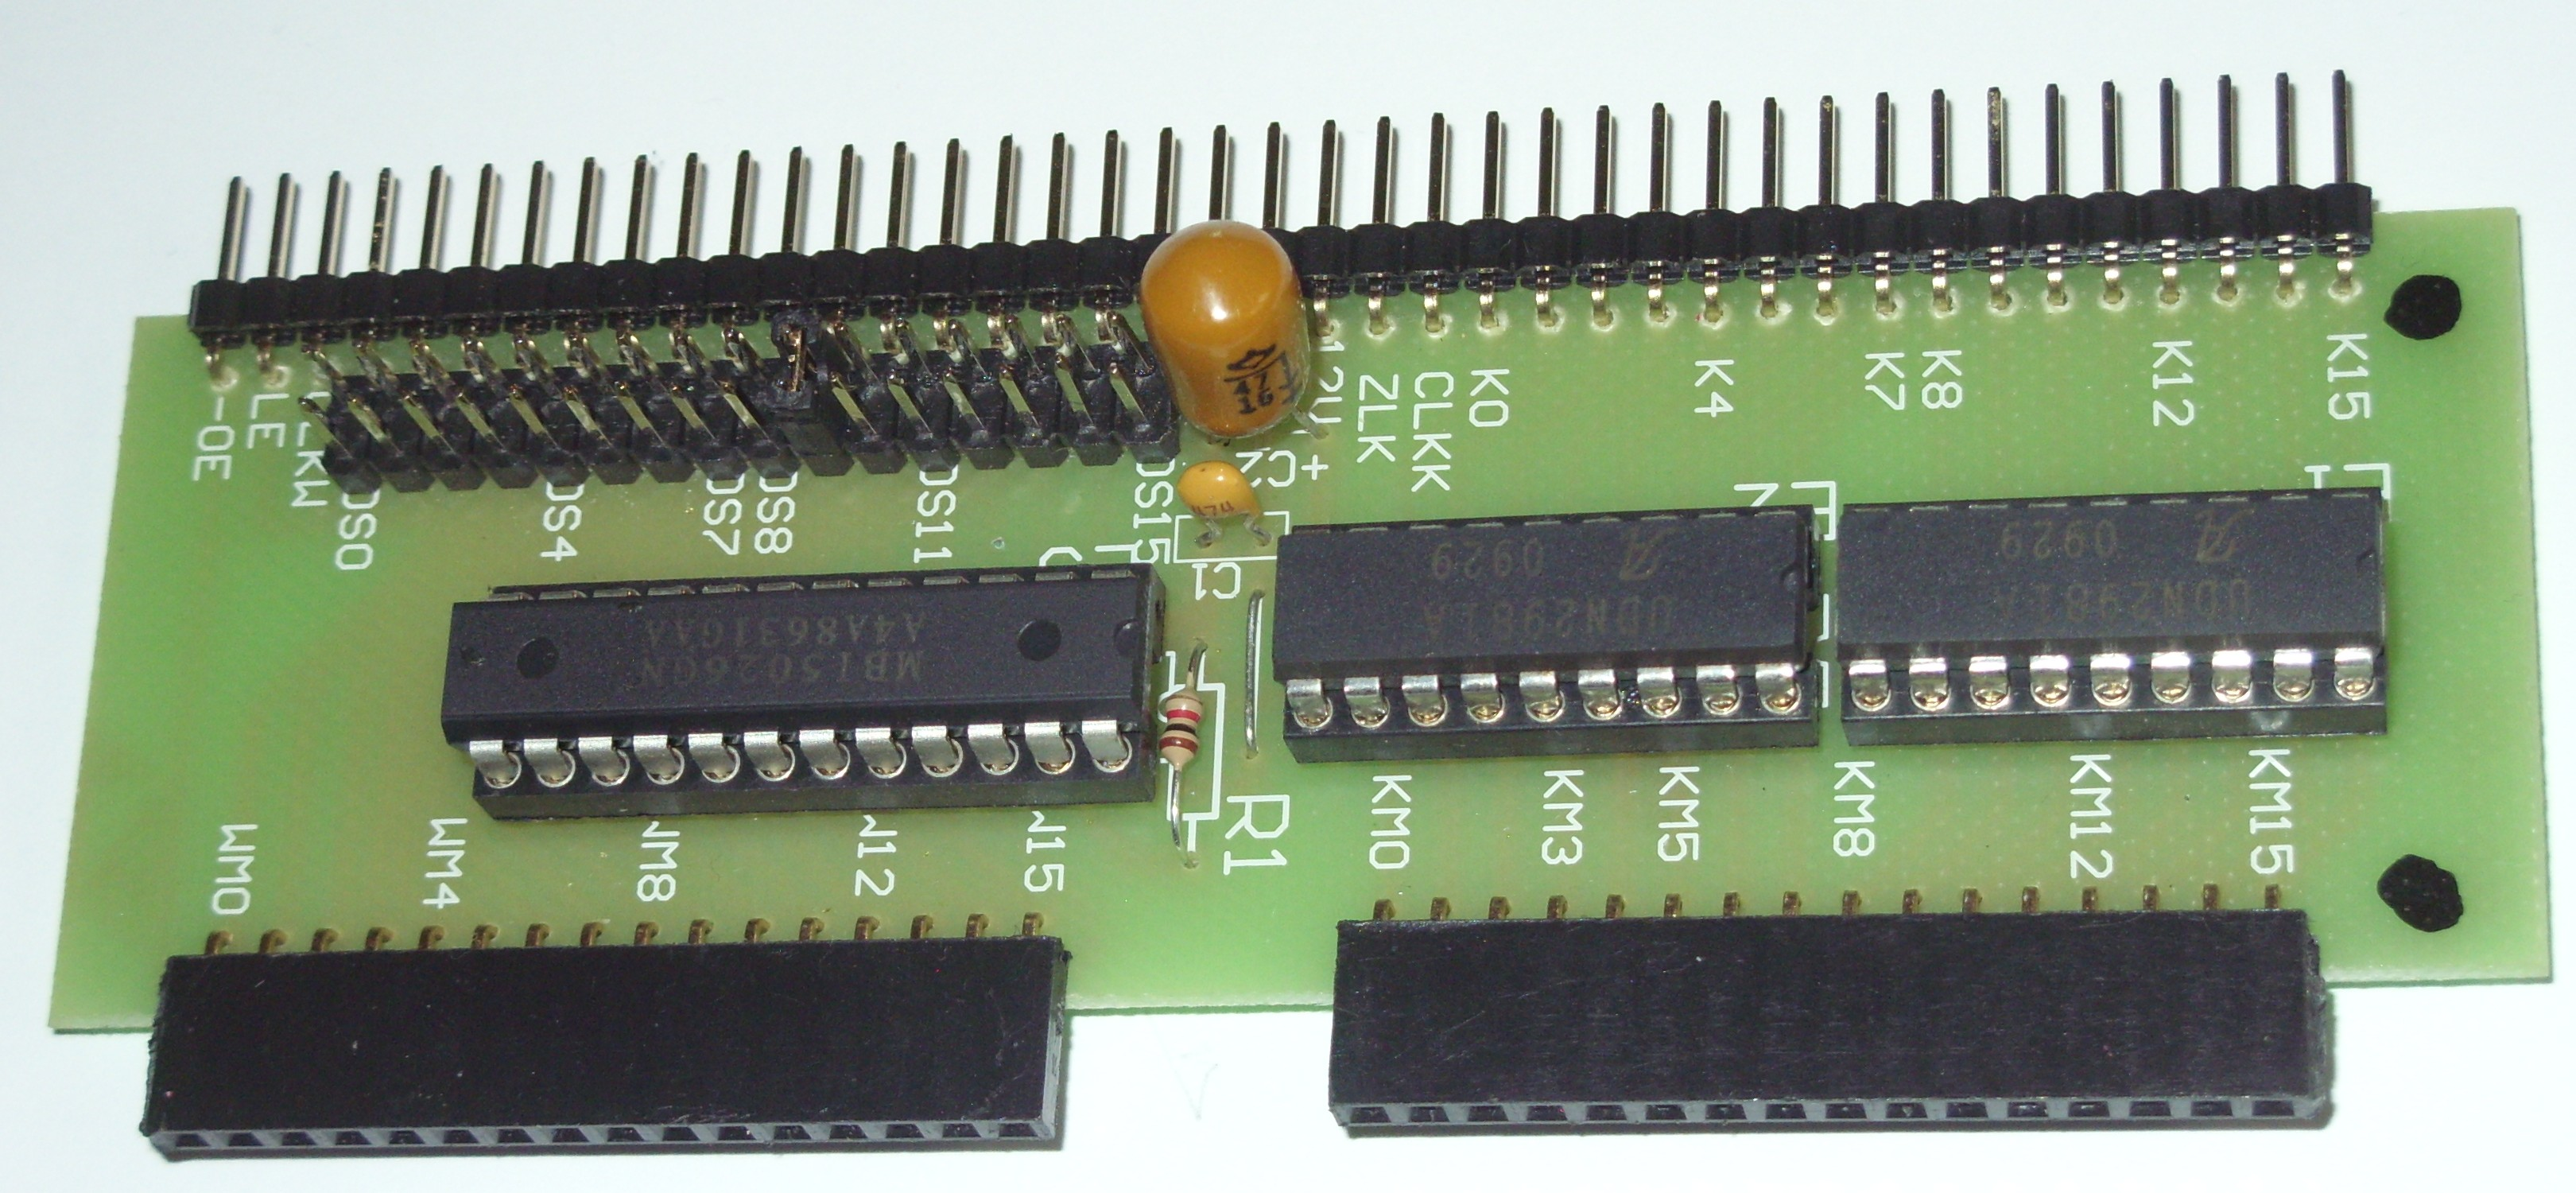
\includegraphics[width=0.8\textwidth]{figures/zdj-driver.jpg}
    \end{center}

    \caption{Zdjęcie modułu drajwera.}
    \label{zdj-driver}
\end{figure}

Układy UDN2981 są cyfrowymi drajwerami mocy wysterowującymi wyjścia od strony napięcia zasilania.  Stan wysoki na wejściu powoduje zwarcie wyjścia z~szyną zasilania. Wydajność sięga $500$ mA na kanał \cite{ds-udn}, co daje duży zapas mocy. Wejścia są kompatybilne ze standardem TTL, co pozwala na bezpośrednie sterowanie ich z~mikrokontrolera. Jeden układ scalony posiada osiem kanałów, w~module użyto dwóch takich układów. Sterują one matrycą diodową od strony anod, służą do wyboru aktualnej kolumny. Sposób sterowania zakłada, że w~danej chwili aktywny będzie tylko jeden kanał z~szesnastu.

Od strony katody matryca sterowana jest za pomocą drajwera MBI5026, który w~swej strukturze, oprócz szesnastu wyjść typu open-collector posiada ograniczenie prądu płynącego przez wyjścia oraz rejestr przesuwny, co pozwala na sterowanie wyjściami za pomocą trzech wyprowadzeń.~Wewnętrzne obwody logiczne dostosowane są do standardu napięć TTL; układ wymaga zasilania $+5$ V, które dostarczane jest przez magistralę.

Maksymalny prąd płynący przez każde z~wyjść O0--015 ustala się rezystorem R1 (rys. \ref{schemat-drivera}) zgodnie ze wzorem:
$$ I_{OUT} = \frac{625}{R_1} \times 28.8 $$
gdzie $I_{OUT}$ to maksymalny prąd płynący przez pojedyncze wyjście układu w~mA \cite{ds-mbi}. W~przyjętym rozwiązaniu układowym ustalono wartość rezystora R1 na $ 1 k\Omega$, co daje prąd wyjściowy rzędu $18$ mA płynący przez pojedynczą diodę LED w~matrycy.

\begin{figure}[tb]
    \begin{center}
       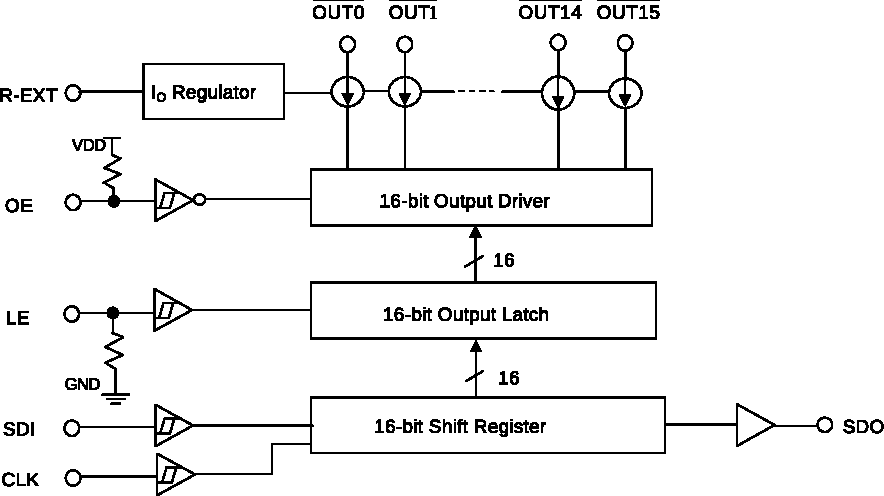
\includegraphics[width=0.8\textwidth]{figures/mbi-block.pdf}
    \end{center}

    \caption{Budowa wewnętrzna układu scalonego MBI5026. Źródło \cite{ds-mbi}.}
    \label{mbi-blokowy}
\end{figure}

\begin{figure}[tb]
    \begin{center}
       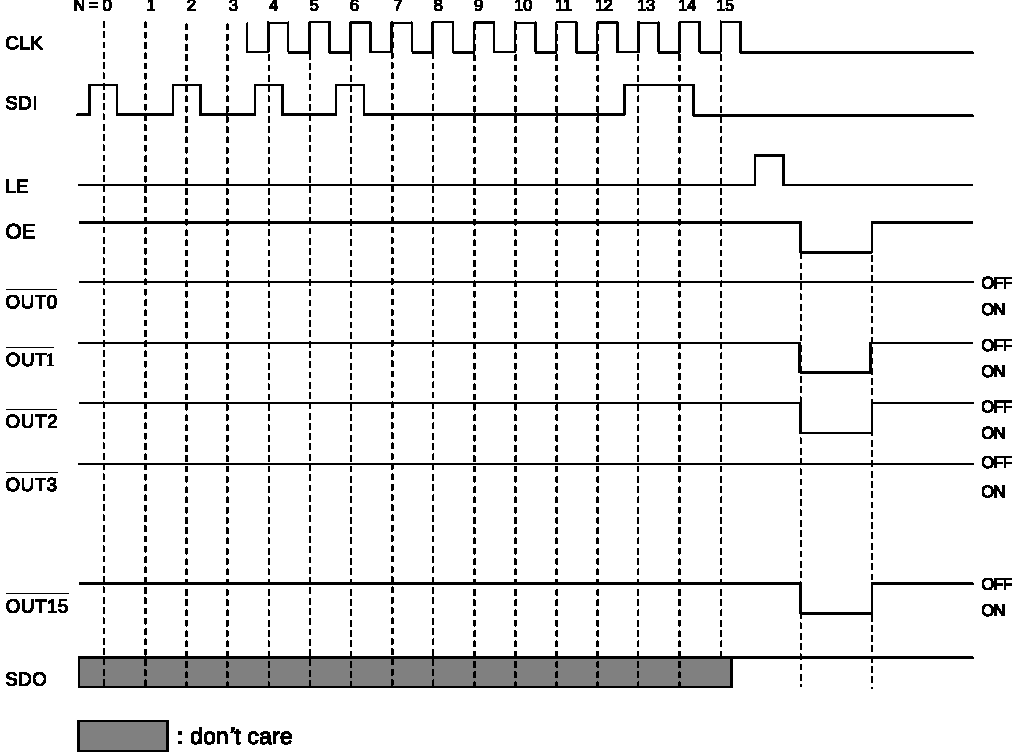
\includegraphics[width=0.8\textwidth]{figures/mbi-timings.pdf}
    \end{center}

    \caption{Wykres czasowy sterowania układem scalonym MBI5026. Źródło \cite{ds-mbi}.}
    \label{mbi-czasy}
\end{figure}

W układzie MBI5026, którego budowę wewnętrzną ilustruje rysunek \ref{mbi-blokowy}, znajduje się 16-bitowy rejestr przesuwny służący do sterowania wyjściami. Zapis odbywa się w~sposób szeregowy tzn. podaje się na wejście SDI stan każdego bitu, zaczynając od najmłodszego. Stan wysoki oznacza wyjście włączone. Zapis następuje na zboczu rosnącym sygnału $CLK$. Dopuszczalna częstotliwość zegara sięga $25$ MHz. Przepisanie zawartości rejestru przesuwnego do rejestru wyjściowego następuje na rosnącym zboczu sygnału LE.~Należy wygenerować taki sygnał, by potwierdzić dane znajdujące się w rejestrze przesuwnym. Wyjścia aktywne są jedynie, gdy wejście $\overline{OE}$ znajduje się w~stanie niskim. Sygnał ten wyprowadzony jest na magistralę i~jest wspólny dla każdego modułu. Wykres czasowy znajduje się na rysunku \ref{mbi-czasy}.

Wejście danych SDI dołączone jest do magistrali przez zestaw zworek PWSM (Pole Wyboru Segmentu Matrycy). Dane są ładowane jednocześnie do każdego z~modułów z~racji wspólnych sygnałów zegarowego i~LE, lecz wejście SDI każdego z~nich dołączone jest do innego wyprowadzenia sterownika, co pozwala na ich indywidualizację. 

\begin{figure}[!p]
    \begin{center}
       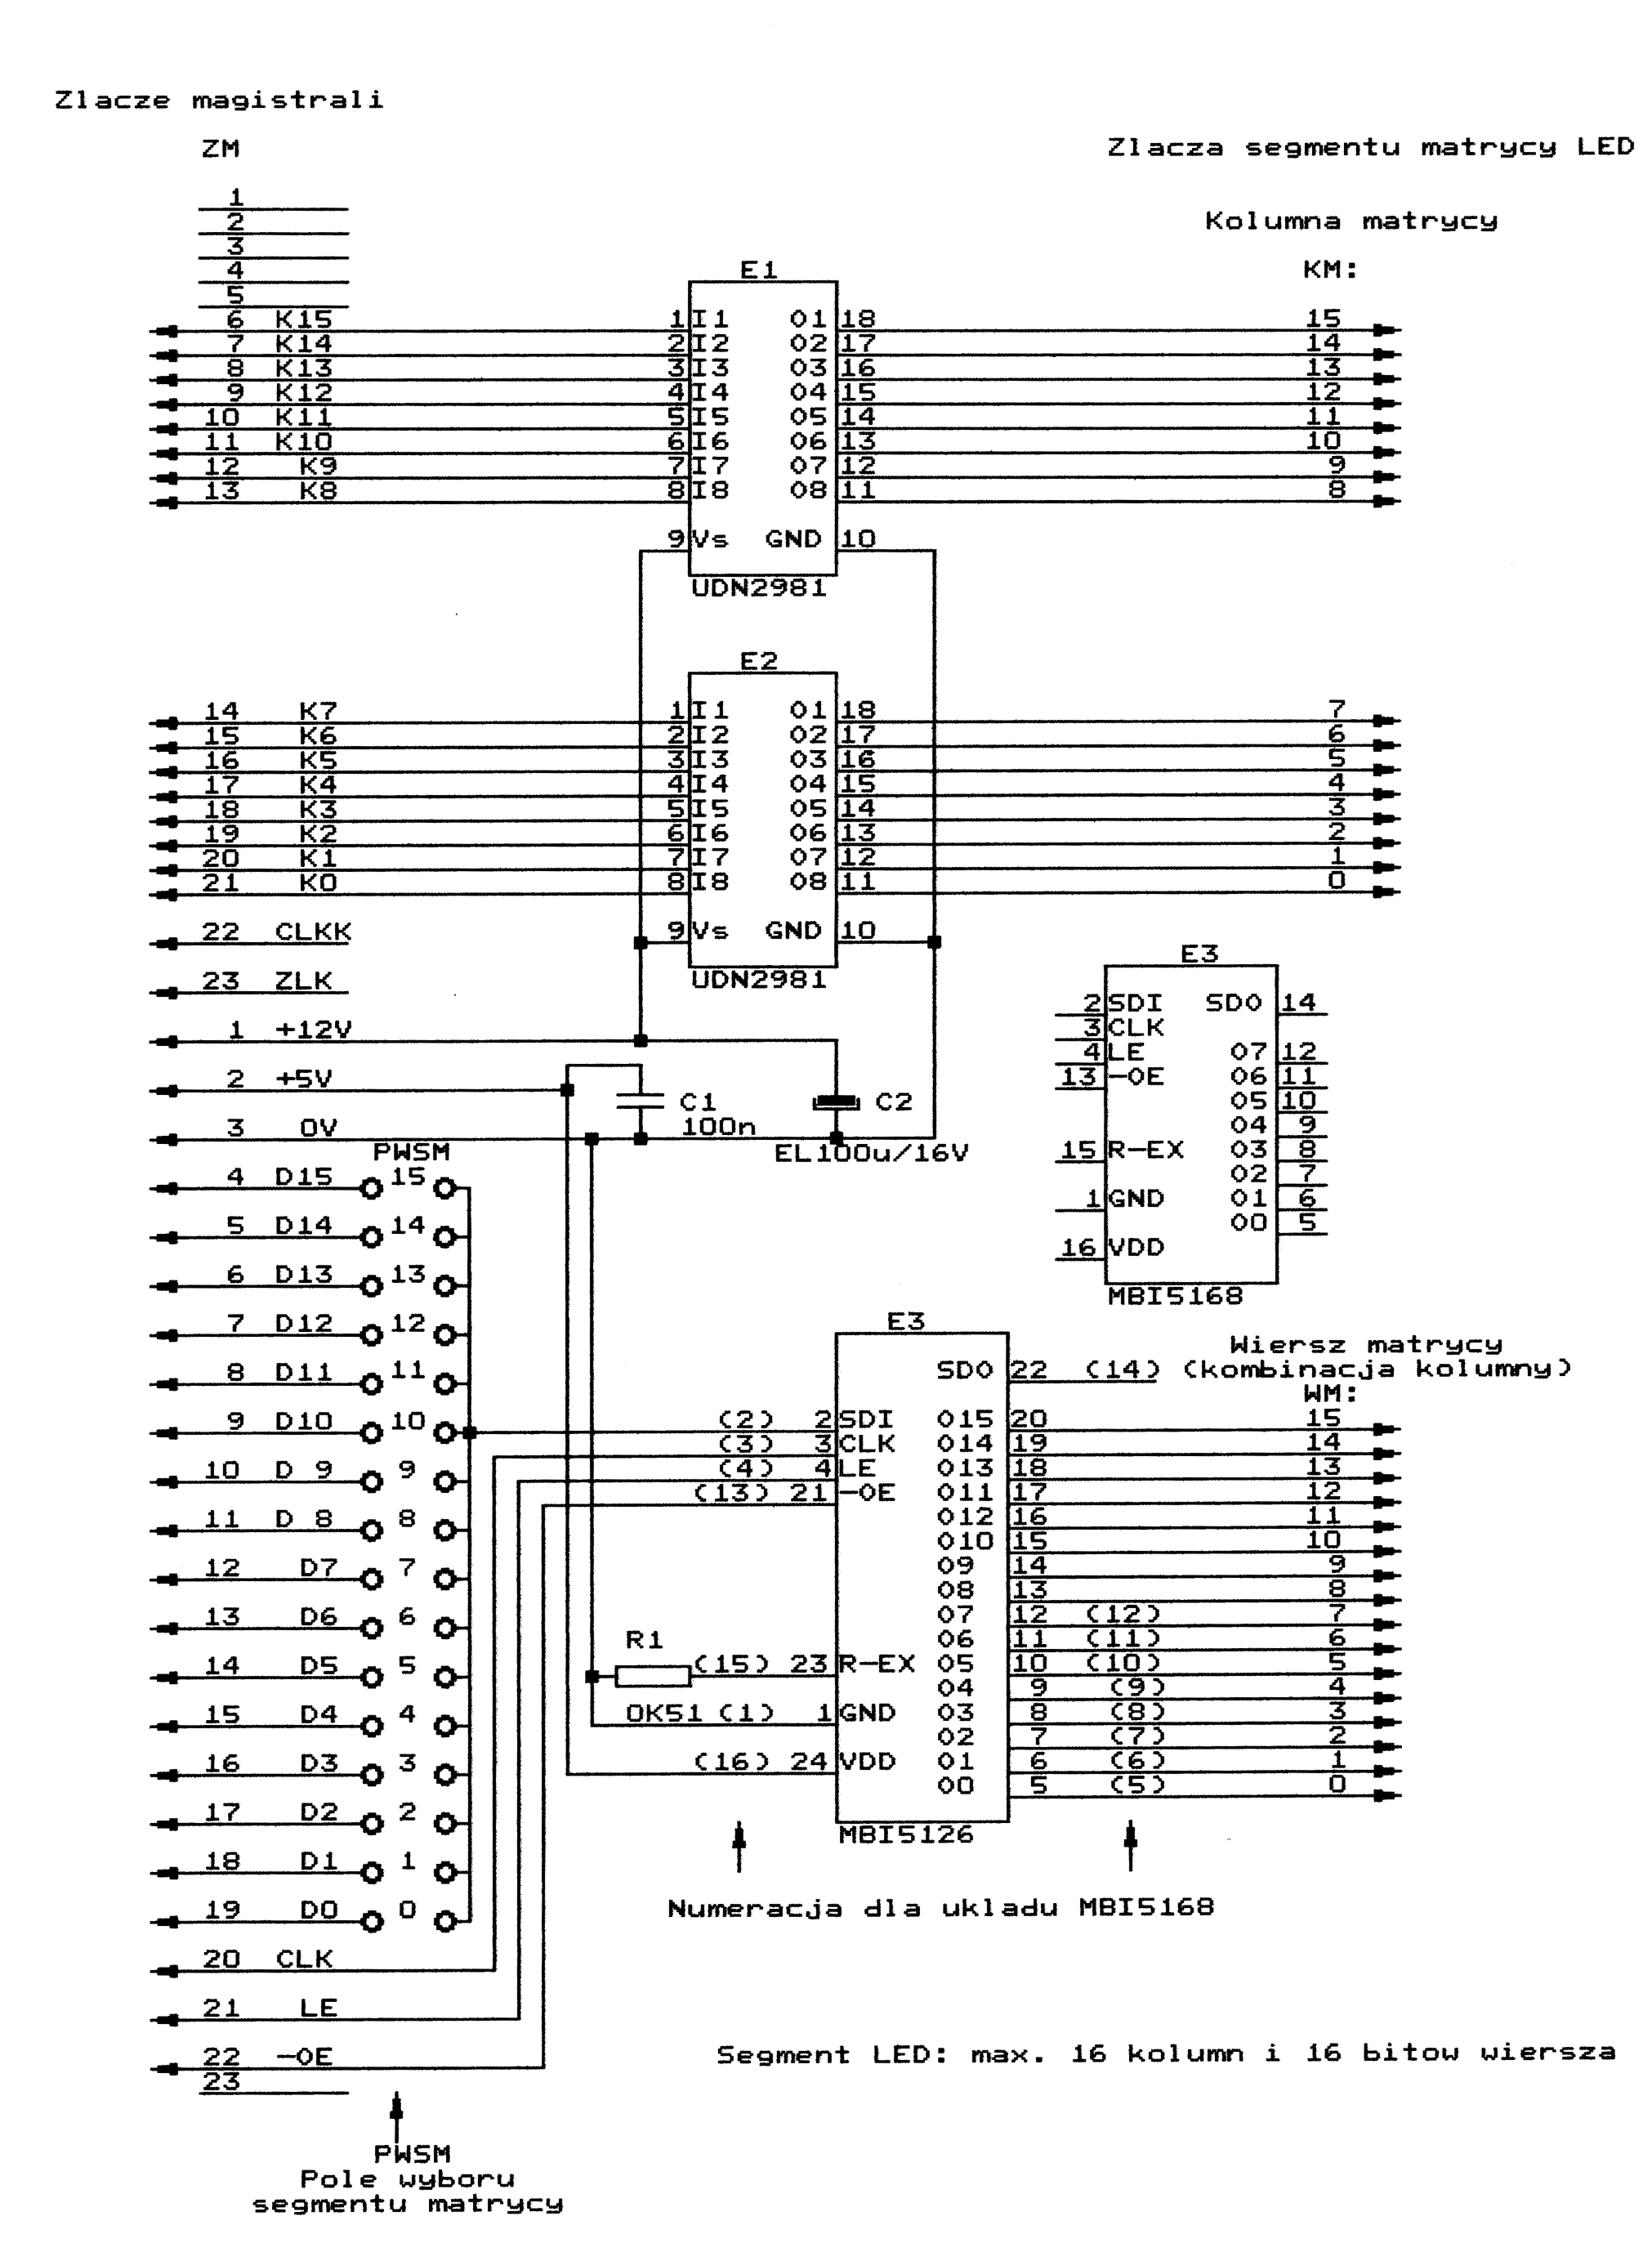
\includegraphics[width=1.1\textwidth]{figures/schemat-driver.png}
    \end{center}

    \caption{Schemat ideowy modułu drajwera.}
    \label{schemat-drivera}
\end{figure}

Magistrala zestawu ma 40 linii, wśród których można wyróżnić następujące grupy:
\begin{itemize}
	\item 16 linii aktywacji kolumny (K0--K15),
	\item 16 linii danych bufora kolumny (D0--D15, jedna linia dla każdego z~modułów),
	\item linia zegara (CLK),
	\item linia potwierdzenia (LE),
	\item linia aktywacji modułów ($\overline{OE}$),
	\item masa, 5~V i~12~V.
\end{itemize}
Pozostałe linie nie są używane. Dokładny opis wyprowadzeń widoczny jest na schemacie (rysunek \ref{schemat-drivera}). 

Zasadniczy algorytm sterowania modułami zaprezentowano poniżej:
\begin{enumerate}
	\item wygaś wszystkie kolumny,
	\item wybierz kolejną kolumnę (1 z~16),
	\item załaduj synchronicznie do bufora danych zawartość kolumny (16 bitów),
	\item potwierdź wypełnienie bufora sygnałem LE,
	\item aktywuj wybraną kolumnę (stan wysoki na jednym z~pinów D),
	\item odczekaj czas odpowiadający przyjętej częstotliwości odświeżania,
	\item wróć do punktu 1.
\end{enumerate}

Punkt pierwszy dodany został z~powodu skończonych czasów wyłączenia buforów znajdujących się w~układzie UDN2981. Zjawisko to objawiało się na ekranie jako widoczny ,,cień''. Czas upływający na szeregowym ładowaniu danych do bufora (punkt 3) pozwala na całkowite wyłączenie bufora UDN2981. 

\textbf{Płytka drukowana magistrali} ma rozmiar $120 \times 113$ mm. Nie zawiera żadnych elementów elektronicznych. Na przeciwległych krawędziach umieszczono 40-pinowe gniazdo i~wtyczkę typu goldpin do łączenia ze sobą wielu modułów. Na środku umieszczono gniazdo goldpin do podłączenia drajwera.

\subsection{Opis sterownika}

Dla istniejącego zestawu wyświetlaczy zaprojektowano moduł sterownika. Umieszczono na nim wszystkie komponenty potrzebne do funkcjonowania urządzenia, z~wyjątkiem zasilacza sieciowego. Dwustronna płytka drukowana z~metalizacją otworów ma wymiary $115 \times 41$ mm.  Schemat ideowy widnieje na rysunku \ref{schemat_sterownika}. Zdjęcia zmontowanego sterownika przedstawiają rysunki \ref{zdj-sterownik-up} i~\ref{zdj-sterownik-down}.

\begin{figure}[tb]
    \begin{center}
       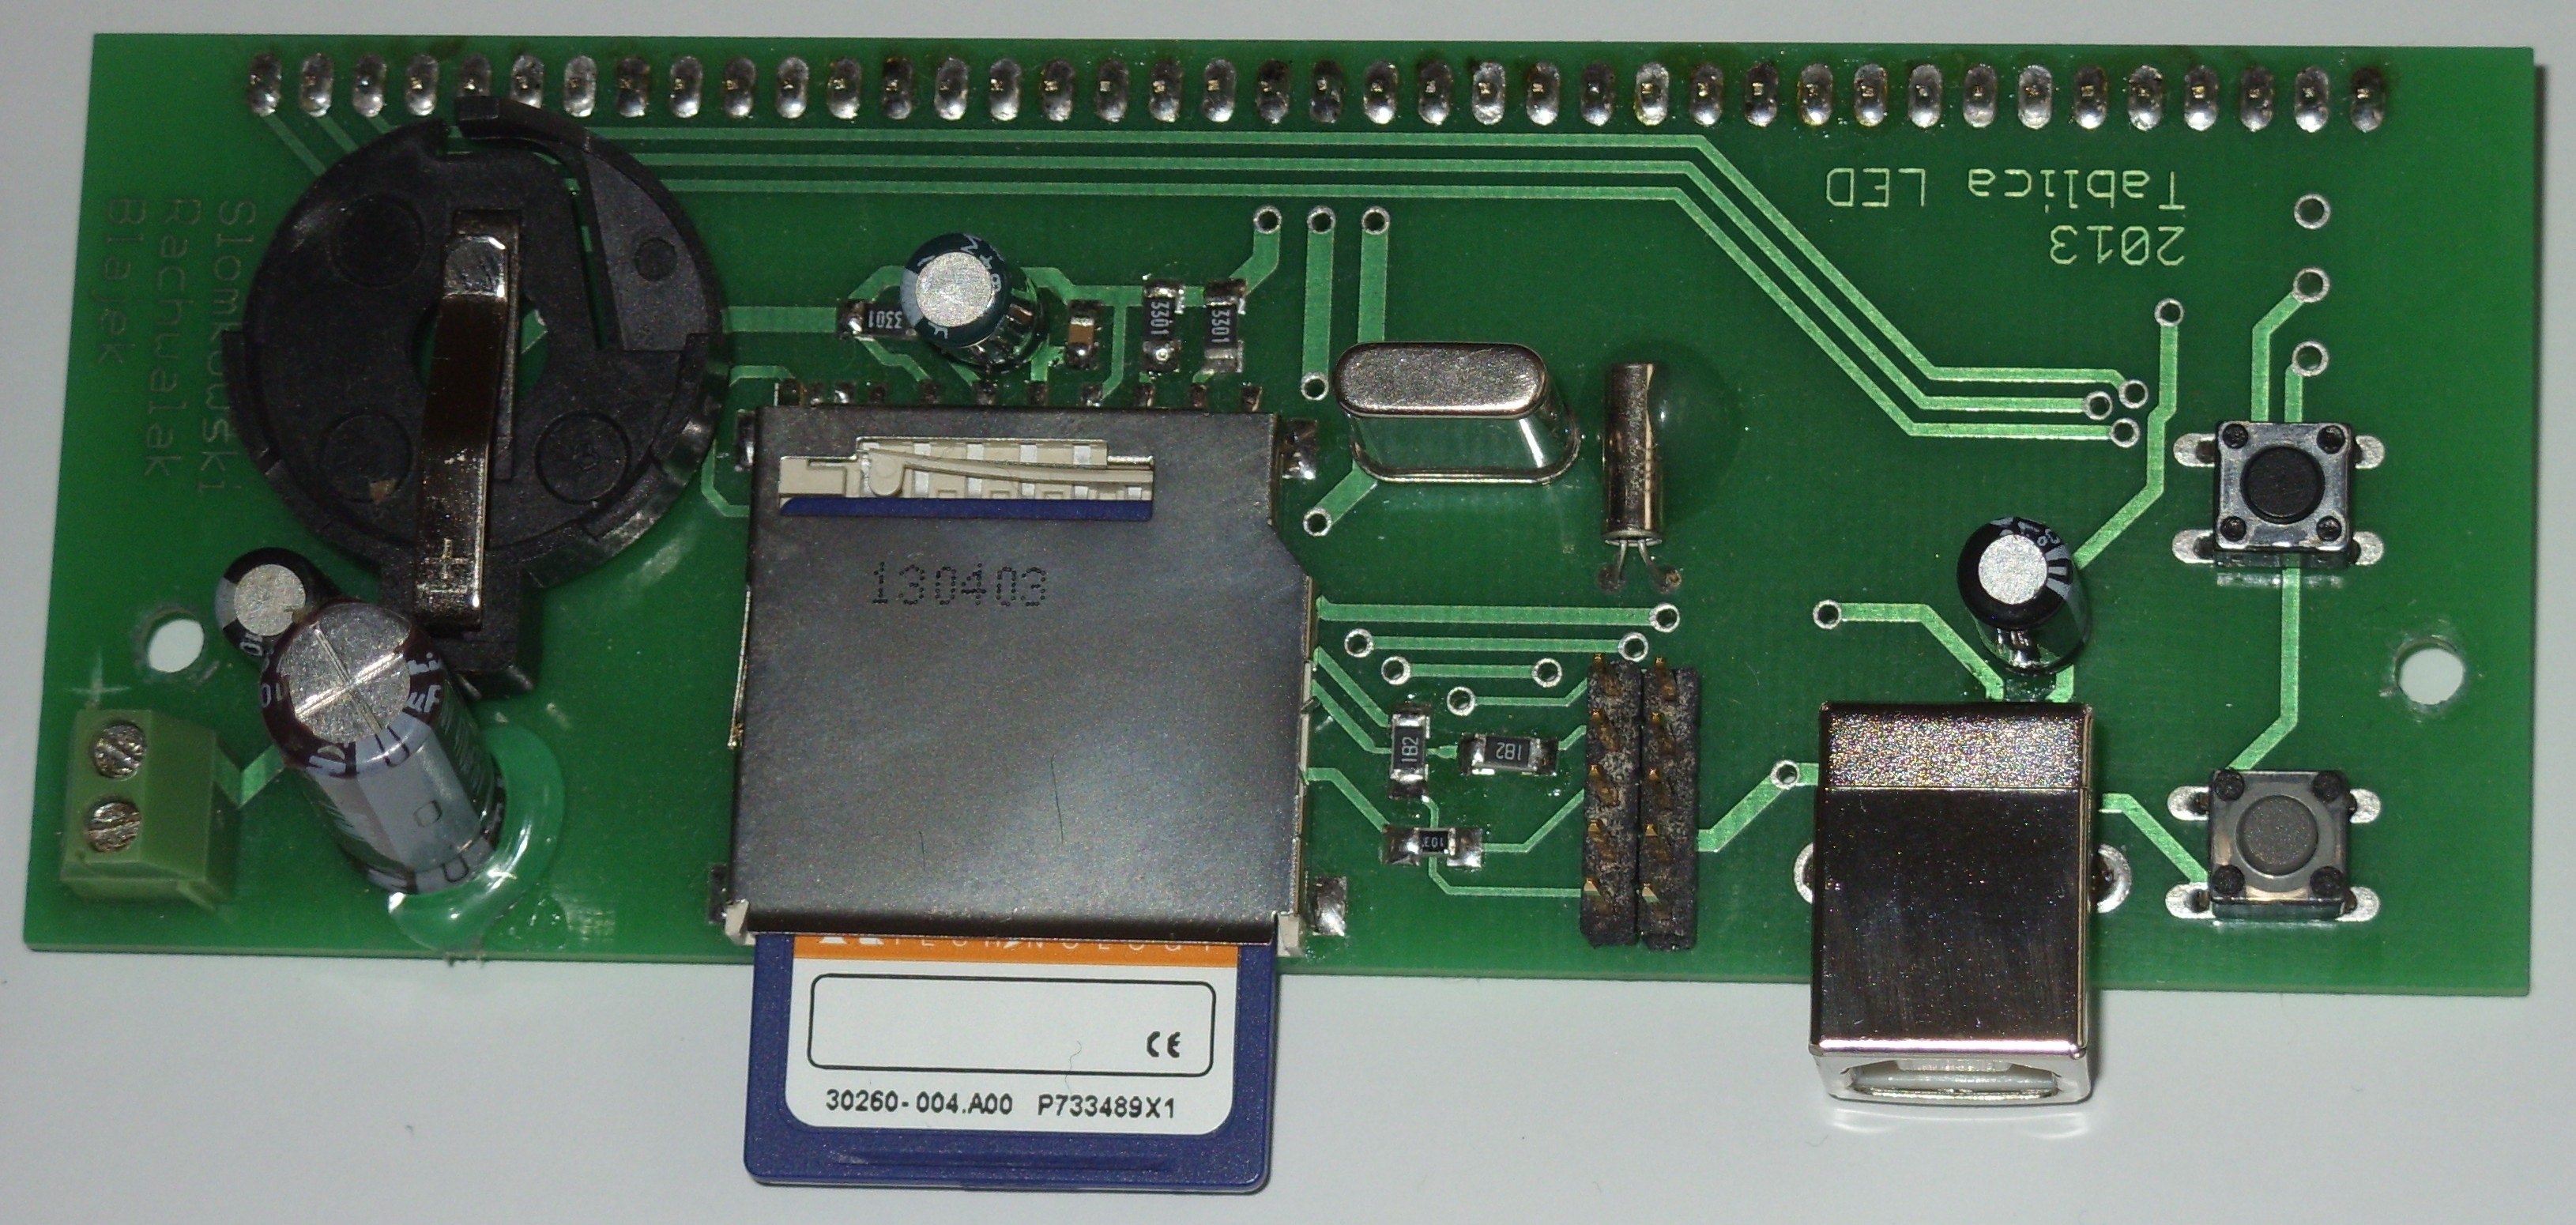
\includegraphics[width=0.8\textwidth]{figures/zdj-sterownik-up.jpg}
    \end{center}

    \caption{Zdjęcie modułu sterownika. Strona górna.}
    \label{zdj-sterownik-up}
\end{figure}

\begin{figure}[tb]
    \begin{center}
       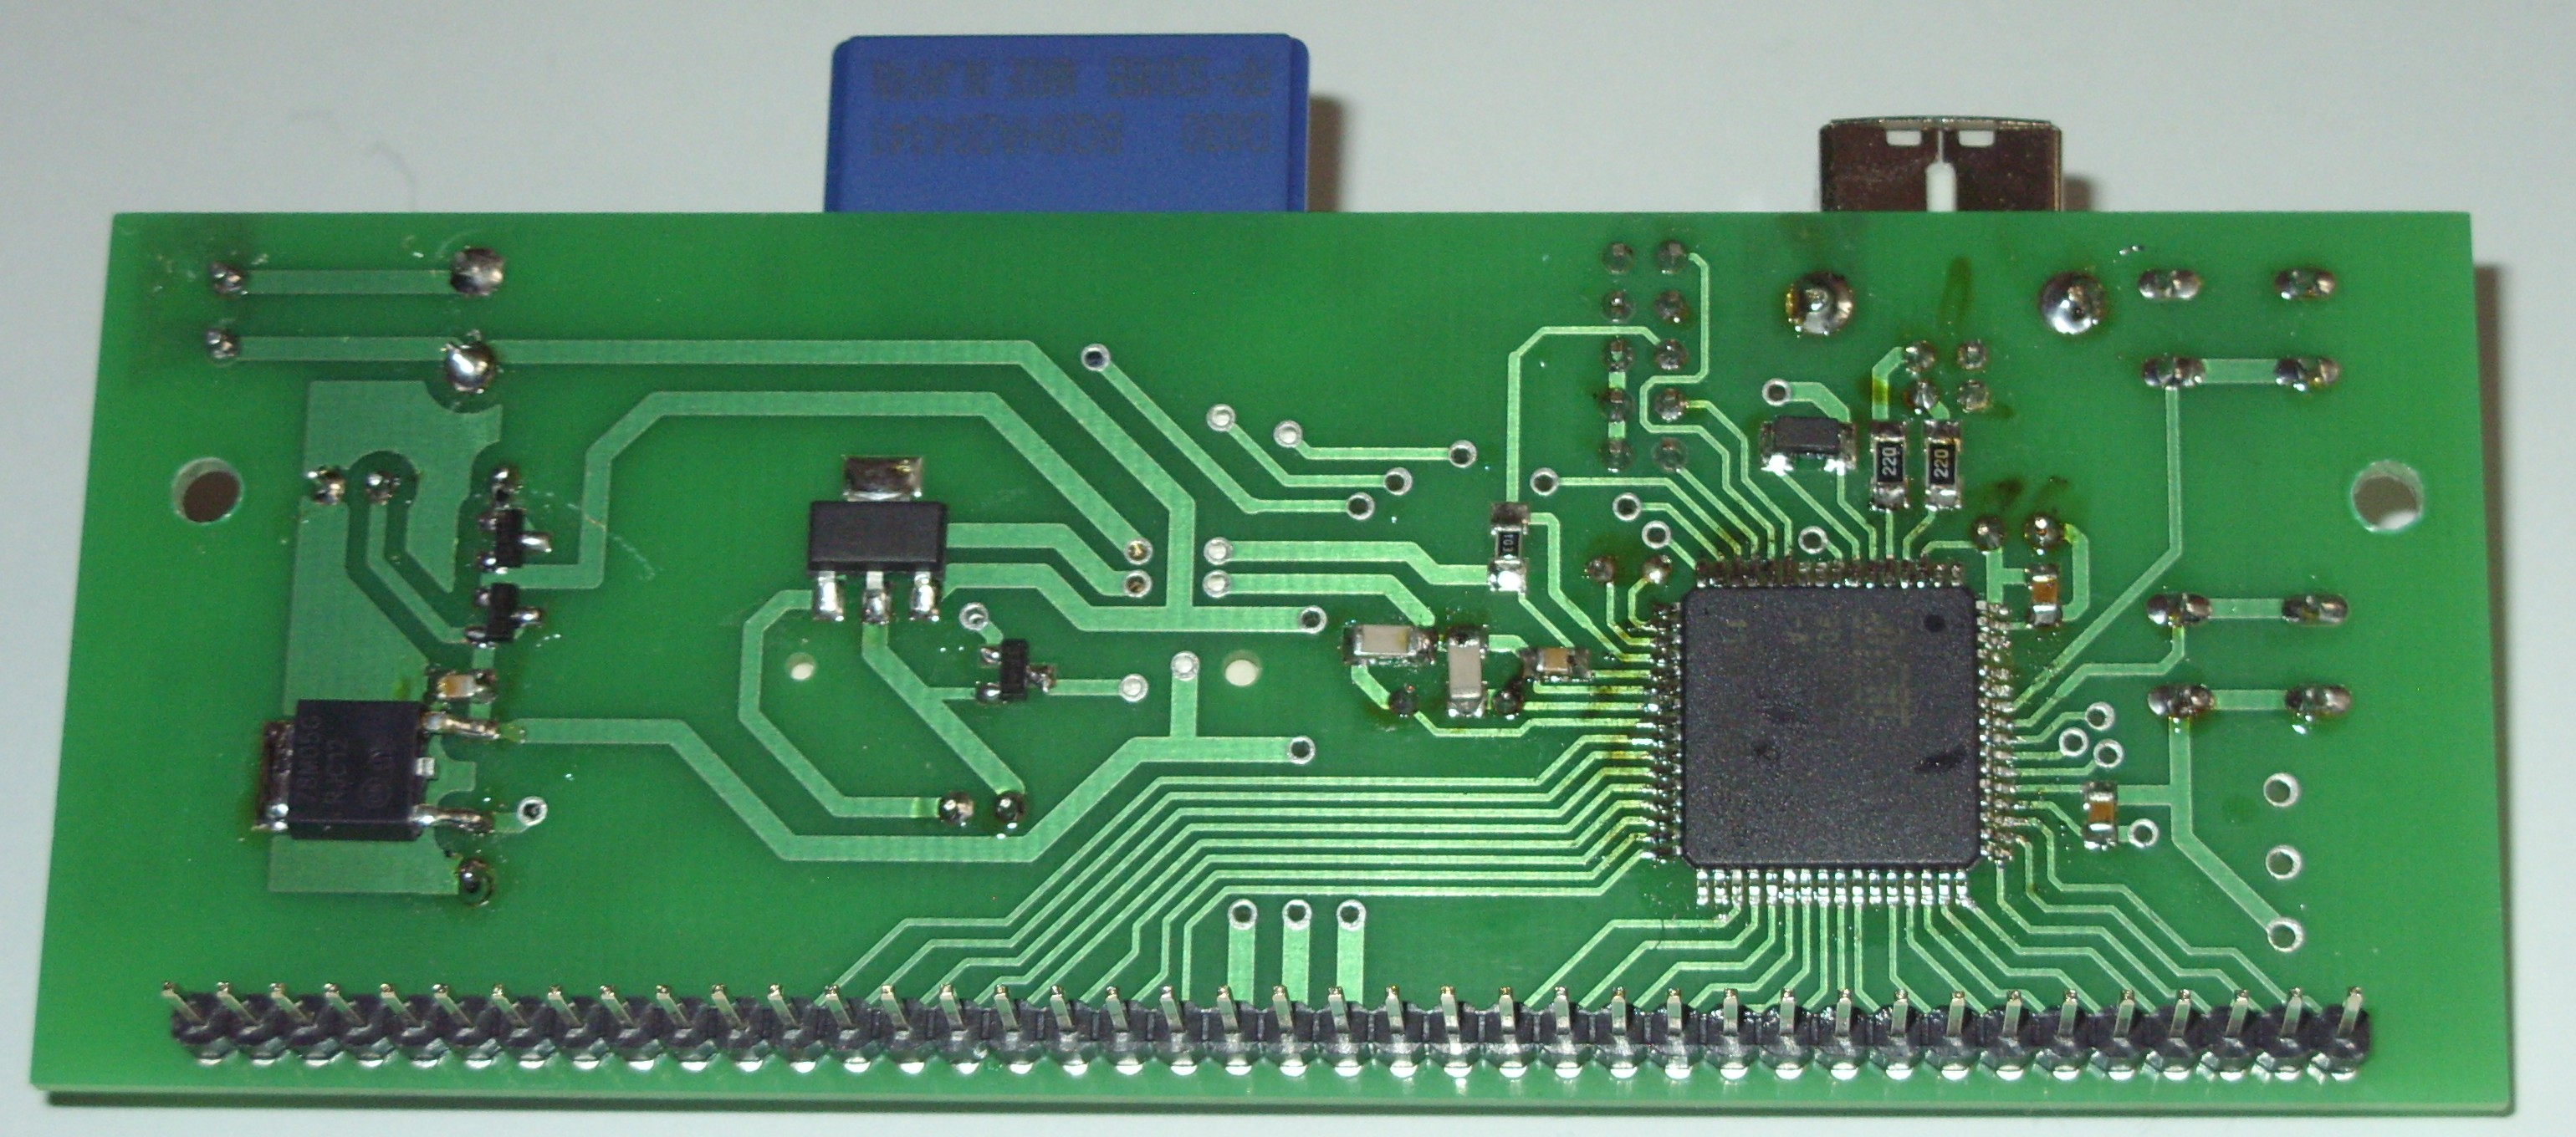
\includegraphics[width=0.8\textwidth]{figures/zdj-sterownik-down.jpg}
    \end{center}

    \caption{Zdjęcie modułu sterownika. Strona dolna.}
    \label{zdj-sterownik-down}
\end{figure}

\begin{sidewaysfigure}
    \begin{center}
       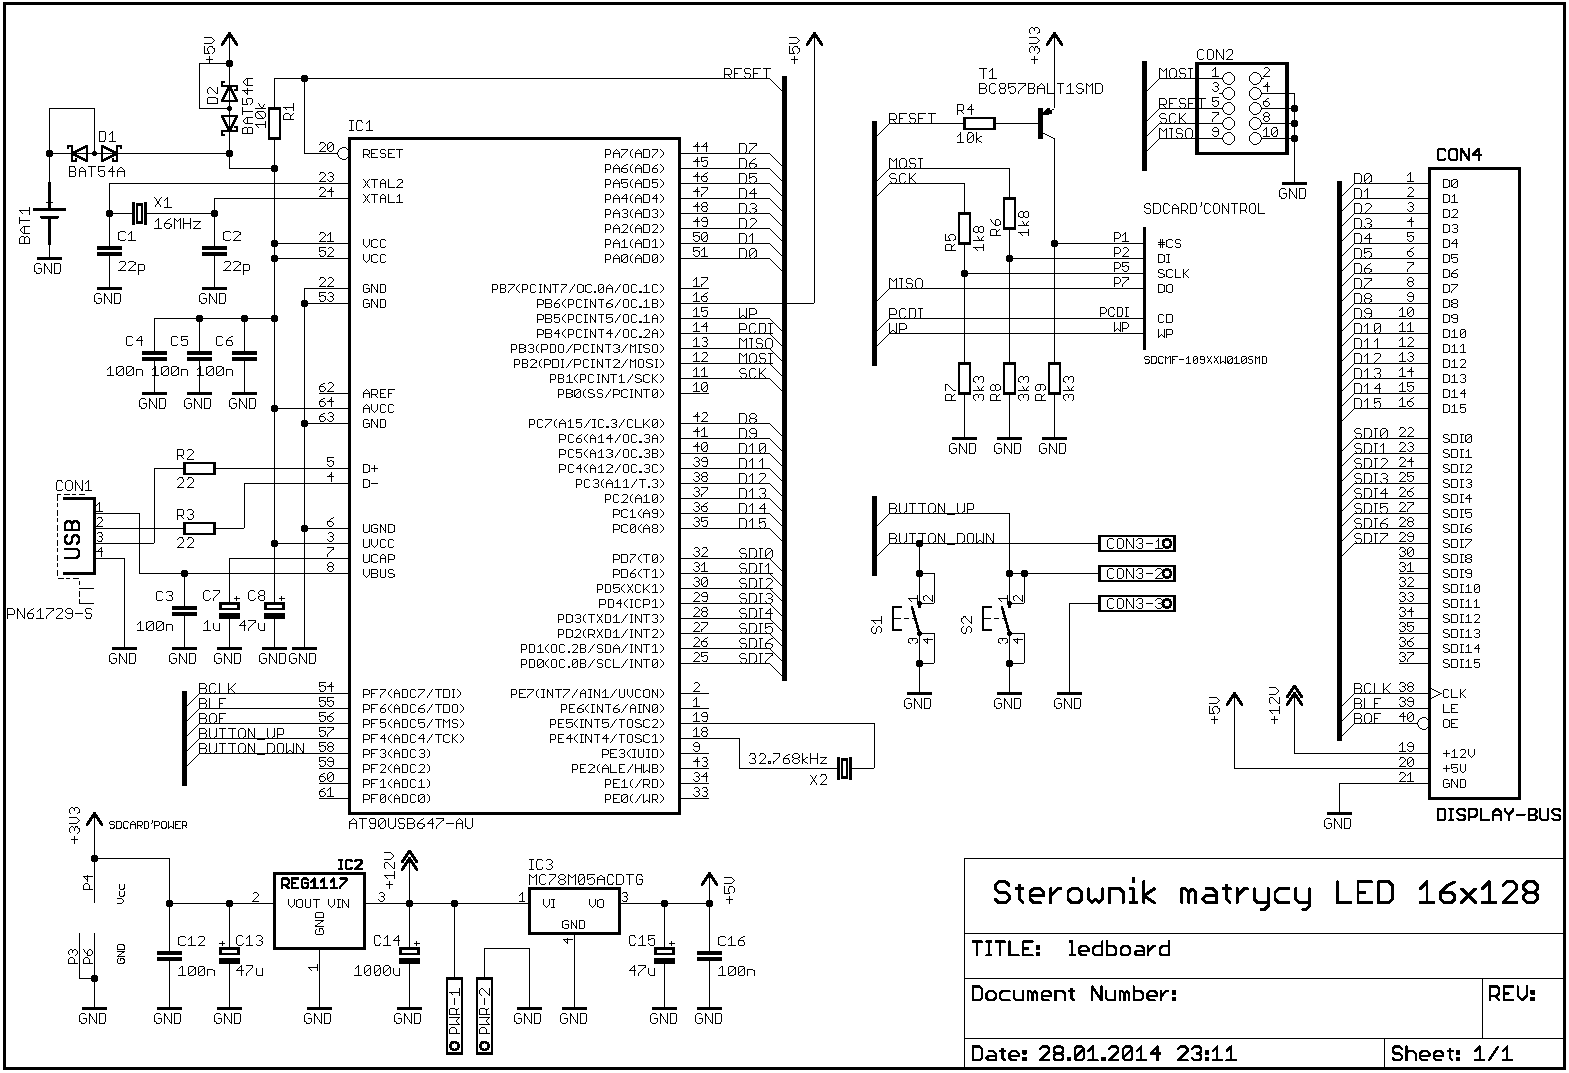
\includegraphics{figures/schemat.pdf}
    \end{center}

    \caption{Schemat ideowy modułu sterownika.}%
    \label{schemat_sterownika}
\end{sidewaysfigure}

\begin{figure}[t]
    \begin{center}
       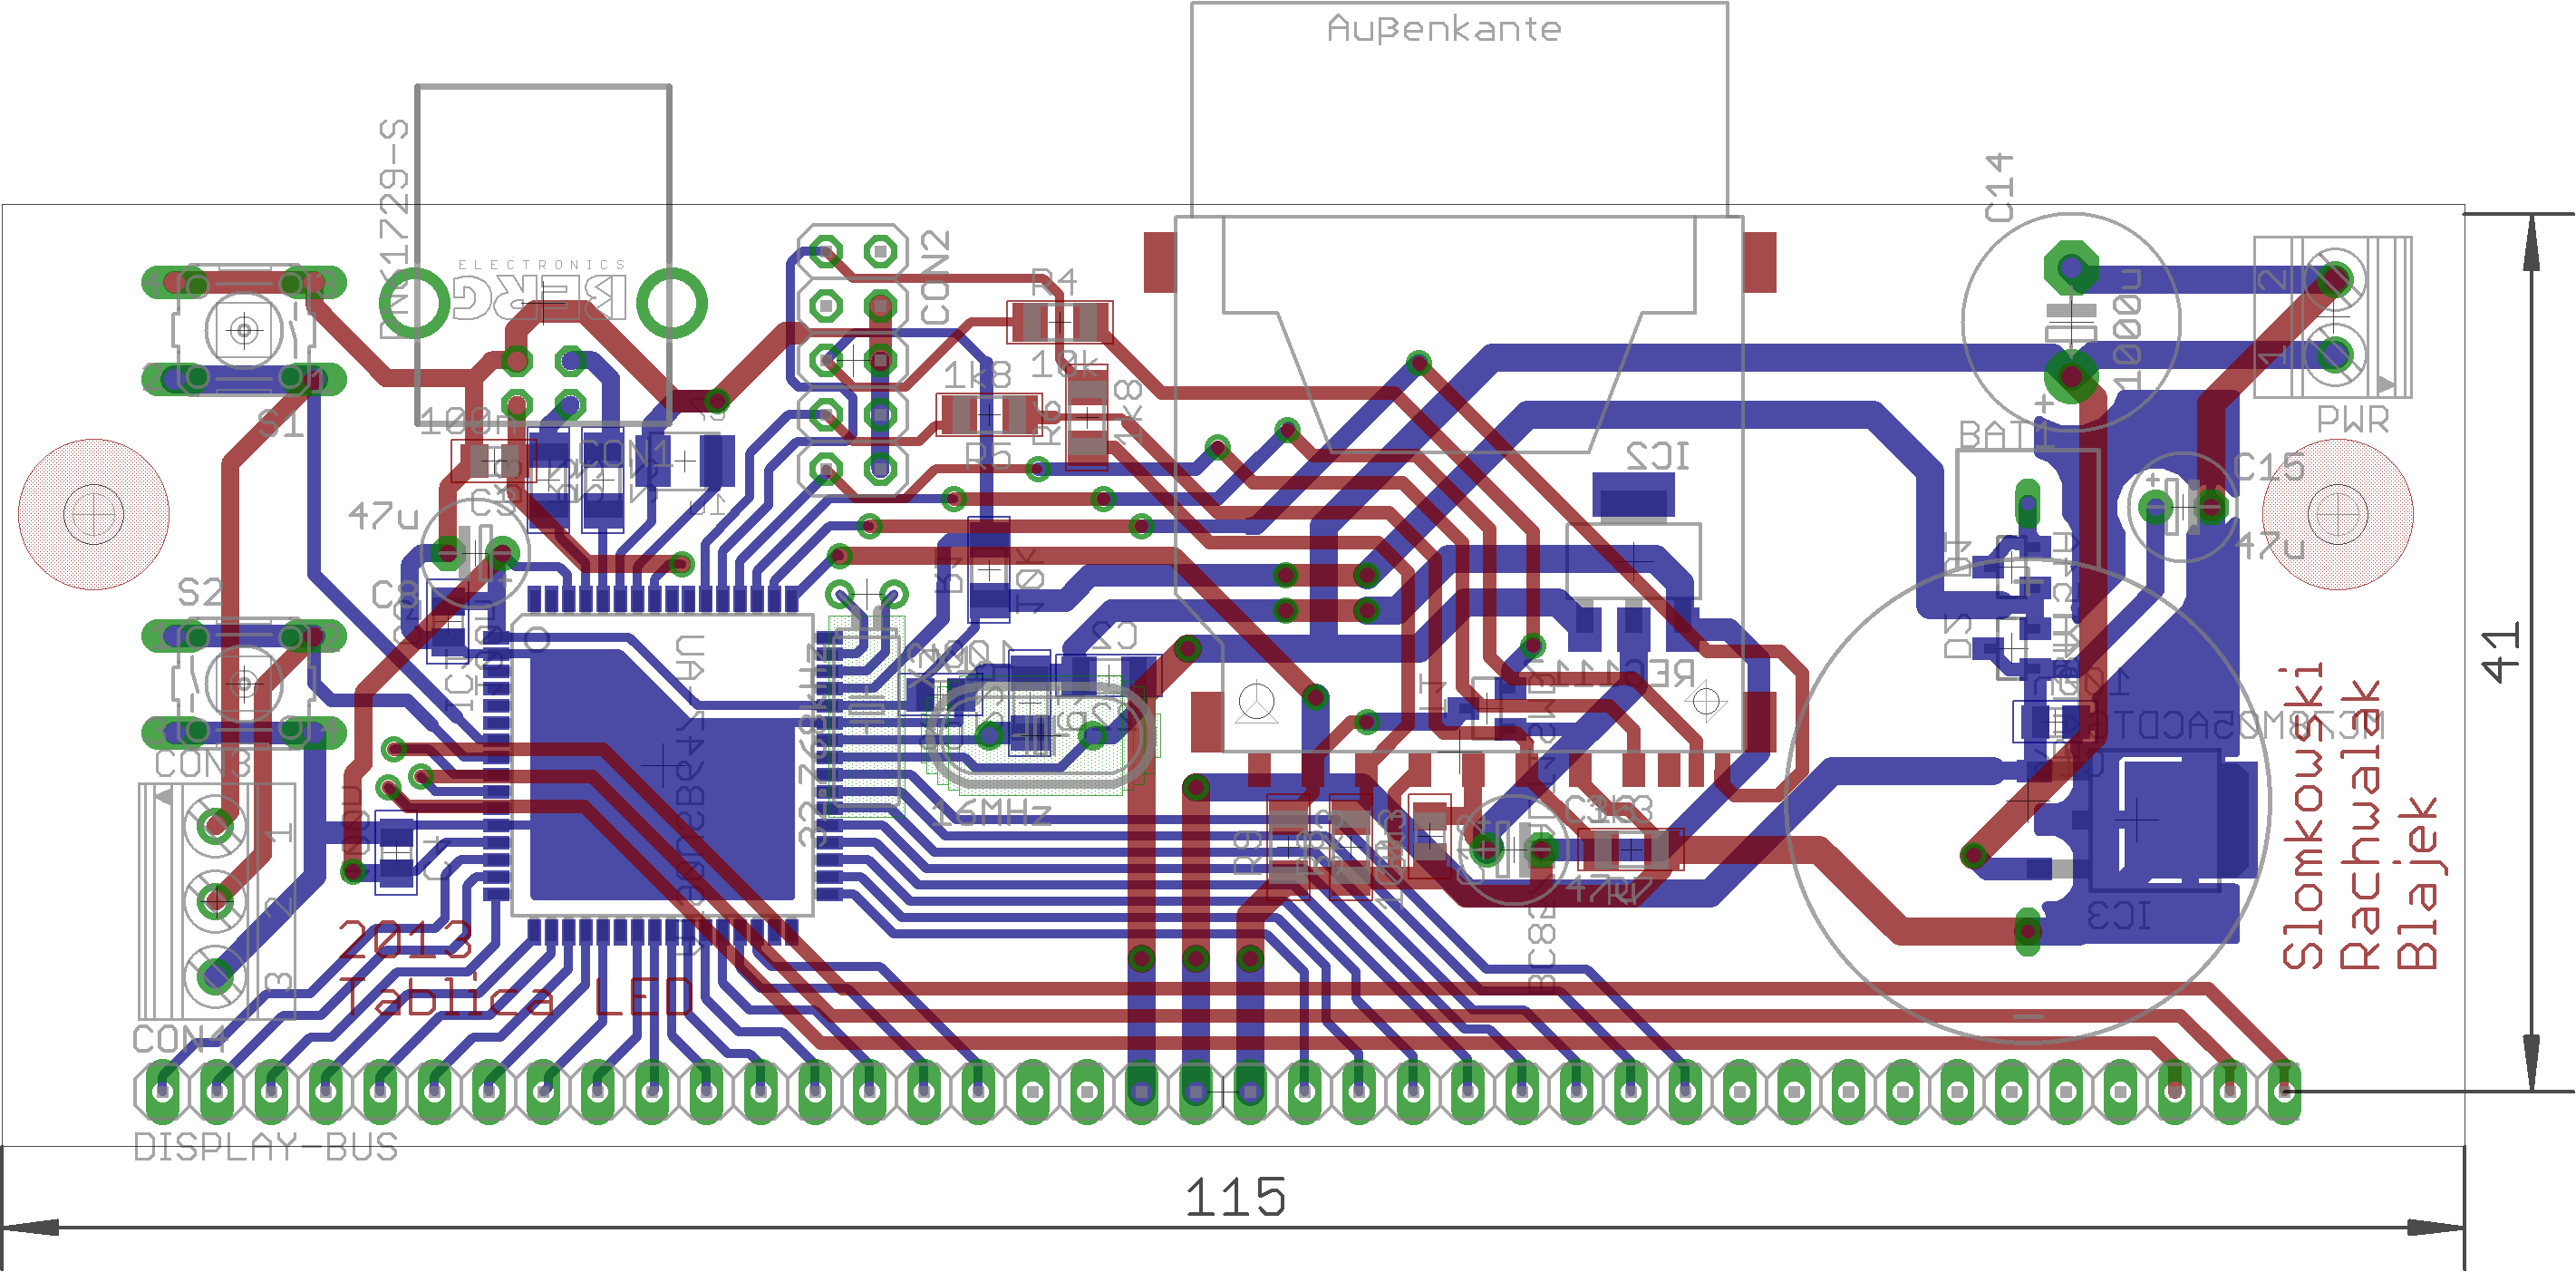
\includegraphics[width=\textwidth]{figures/layout.png}
    \end{center}

    \caption{Wzór ścieżek płytki drukowanej modułu sterownika.}%
    \label{layout_sterownika}
\end{figure}

Na płytce umieszczono następujące elementy:
\begin{itemize}
	\item mikrokontroler AT90USB647 wraz z~komponentami niezbędnymi do pracy, jak rezonatory kwarcowe i~kondensatory odsprzęgające,
	\item gniazdo USB typu B,
	\item gniazdo karty SD,
	\item podstawka baterii CR2032 podtrzymująca pracę zegara czasu rzeczywistego w~razie awarii zasilania,
	\item złącze ISP typu goldpin w~standardzie STK200 służące do programowania mikrokontrolera w~układzie docelowym,
	\item dwa przyciski typu microswitch wraz ze złączem śrubowym,
	\item stabilizatory napięcia 5~V i~3,3~V odpowiednio dla mikrokontrolera i~karty SD.
\end{itemize}

Płytkę drukowaną, której wzór ścieżek zaprezentowano na rysunku \ref{layout_sterownika}, zaprojektowano w~niekomercyjnej wersji pakietu Eagle firmy Cadsoft. Płytka jest dwuwarstwowa, z~metalizacją otworów. Większość użytych elementów jest w~obudowach dostosowanych do montażu powierzchniowego. W~celu lepszego odprowadzania ciepła od stabilizatora IC3, umieszczono wokół niego pole miedzi, do którego przylutowana jest obudowa. Ścieżki masy i~zasilania mają grubość $1.27$ mm; grubość pozostałych jest mniejsza i~zależy od wygody prowadzenia danego sygnału.

Moduł został zaprojektowany w~ten sposób, by łatwe było jego zamontowanie na istniejącej płytce magistrali i~umieszczenie całości w~obudowie. Wzdłuż zewnętrznej krawędzi umieszczono 40-pinowe złącze magistrali danych. Po przeciwnej stronie umiejscowione zostały złącza karty SD i~USB.~Płytka montowana jest do magistrali przy pomocy dwóch śrub M3 na tulejkach dystansowych. Od strony wewnętrznej moduł wsparty jest na złączu goldpin magistrali danych. Z~racji takiej ilości pinów połączenie to posiada możliwość przenoszenia również sił mechanicznych powstających podczas normalnego użytkowania, jak wkładanie i~wykładanie karty SD oraz podłączenie wtyku USB.

Centralnym elementem modułu jest mikrokontroler jednoukładowy z~rodziny AVR firmy Atmel, AT90USB647. Jest on wyposażony w~$64$ kB pamięci FLASH i~$4$ kB RAM.~Jak sugeruje oznaczenie, jest wyposażony w~sprzętowy kontroler USB typu device, co pozwoliło na łatwą implementację komunikacji z~komputerem PC przy użyciu biblioteki LUFA i~klasy Mass Storage. Mikrokontroler posiada 64-wyprowadzeniową obudowę typu TQFP64 dostosowaną do montażu powierzchniowego. Bardziej szczegółowe omówienie użytego mikrokontrolera zamieszczono w~rozdziale teoretycznym pracy. Użyte moduły mikrokontrolera zostały wyszczególnione w~sekcji poświęconej oprogramowaniu.

Choć magistrala umożliwia wysterowanie maksymalnie szesnastu modułów wyświetlaczy, ograniczona ilość wyprowadzeń wymusiła ograniczenie ich liczby do ośmiu. Linie odpowiadające za wybór kolumny zajmują całe porty A~i~C. Z~uwagi na łatwość prowadzenia ścieżek linie D0-D7 dołączone są do portu A~rosnąco, z~kolei D8-D15 --- malejąco. Program mikrokontrolera dokonuje odpowiedniego odwrócenia kolejności bitów tak, by wszystkie 16 linii było odwzorowane na pojedynczą 16-bitową zmienną.

Port D w~całości zajęty jest przez linie danych dołączone do buforów umieszczonych w~modułach wyświetlaczy. Oprócz tego do wyprowadzeń portu F dołączone są sygnały CLK, LE i~OE.~Sterownik nie odczytuje żadnych danych z~modułów wyświetlaczy; wszystkie wyżej wymienione porty skonfigurowane są jako standardowe wyjścia i~nie wykorzystują alternatywnych funkcji wyprowadzeń mikrokontrolera.

Mikrokontroler wyposażony jest w~sprzętowy interfejs SPI, który udostępnia również możliwość zaprogramowania mikrokontrolera w~układzie docelowym (ISP). By korzystać z~tej możliwości, na płytce umieszczono złącze goldpin $2 \times 5$, zgodne ze standardem STK200. Umożliwiło to wykorzystywanie popularnych programatorów. Programowanie odbywa się przy wymuszonym stanie niskim na wejściu RESET mikrokontrolera.

Karta SD pracuje z~poziomem napięć $3.3$ V, natomiast mikrokontroler --- $5$ V.~Niezbędne stało się więc zastosowanie konwertera napięć. Wykorzystano proste rozwiązanie oparte o~dzielniki napięcia. Napięcie dzielone jest tylko na wyprowadzeniach MOSI (Master Output Slave Input) i~SCK (zegar), gdyż tylko na nich występuje $5$ V w~stanie wysokim. Pozostałe wyprowadzenia mają charakter wejść, więc tego typu dzielniki nie są wymagane.

Obwód z~tranzystorem T1 (rys. \ref{schemat_sterownika}) wymusza stan wysoki na wejściu $\overline{CS}$ karty SD, podczas programowania mikrokontrolera przez złącze ISP.~Powoduje to odłączenie karty SD od magistrali, co zapobiega konfliktom. Gniazdo karty SD, oprócz interfejsu komunikacyjnego udostępnia sygnały CD i~WP, które informują odpowiednio o~obecności karty i~włączonej ochronie zawartości. Zaimplementowane są one jako zwyczajne styki mechaniczne, dlatego niezbędne stało się podciąganie tych wejść do napięcia zasilania, tak jak w~przypadku ze zwykłymi przyciskami.

Komunikację z~komputerem PC umożliwia umieszczone na płytce gniazdo USB typu B.~Dzięki zintegrowanemu z~mikrokontrolerem sprzętowym interfejsem USB typu device zbędne stało się stosowanie zewnętrznych układów scalonych. Gniazdo połączone jest z~mikrokontrolerem dwoma rezystorami o~wartości $22$ $\Omega$, zgodnie z~notą katalogową \cite{ds-avr}. Kondensator C7 zapewnia odpowiednią filtrację napięcia $3.3~V$ generowanego przez wewnętrzną przetwornicę. Zgodnie z~zaleceniami, ścieżki między mikrokontrolerem, rezystorami i~gniazdem poprowadzono w~możliwie najkrótszy i~najbardziej symetryczny sposób. Poprawia się przez to tłumienie zakłóceń wspólnych.


Sygnał zegarowy na potrzeby mikrokontrolera generuje jego wewnętrzny oscylator wykorzystujący rezonator kwarcowy X1 o~częstotliwości pracy $16$ MHz. Co prawda mikrokontroler posiada wbudowany oscylator RC o~częstotliwości $8$ MHz, jednak ostry reżim czasowy magistrali USB wymusza użycie rezonatora kwarcowego. Wybór takiej, a~nie innej częstotliwości podyktowany został uzyskaniem możliwie dużej wydajności mikrokontrolera. Maksymalna obsługiwana częstotliwość gwarantowana przez producenta to $20$ MHz, jednak kontroler USB wymaga taktowania $48$ MHz. Wewnętrzny układ pętli fazowej powiela częstotliwość zegarową do wymaganej wartości. Racjonalne więc okazało się użycie $16$ MHz, gdyż $3 \times 16 = 48$.

Ośmiobitowy Timer2 mikrokontrolera użyto jako generator zegarowy o~okresie $1$ s. Wykorzystano dostępny tryb asynchroniczny pracy zegara, by uniezależnić się od głównego sygnału taktującego. Timer taktowany jest własnym generatorem używającym zewnętrznego rezonatora kwarcowego $32.768$ kHz, znanego powszechnie jako kwarc zegarkowy. Timer został skonfigurowany tak, by generował przerwanie co sekundę. Wyliczanie czasu i~daty, obsługa dat przestępnych itd. zostały zrealizowane programowo zgodnie z~instrukcją \cite{an-134}. Użycie trybu asynchronicznego pracy timera pozwoliło na przełączanie mikrokontrolera w~tryb niskiego poboru energii w~przypadku wykrycia zaniku głównego napięcia zasilania. W~trybie tym nie pracują żadne podsystemy mikrokontrolera z~wyjątkiem timera 2, co ogranicza pobór prądu z~baterii. Po wygenerowaniu przerwania przez timer, co ma miejsce co sekundę, mikrokontroler ,,budzi się'' na czas potrzebny do aktualizacji struktury przechowującej aktualny czas, po czym na powrót jest usypiany.

Użytkownik obsługuje urządzenie za pomocą dwóch monostabilnych przycisków zwiernych, umownie oznaczonych UP i~DOWN.~Zostały one umieszczone na panelu bocznym, połączone ze sterownikiem przewodem. Na samej płytce drukowanej umieszczono dwa przyciski typu \textit{microswitch}, które przydatne były na etapie konstrukcji urządzenia, gdy nie posiadało ono jeszcze obudowy. Przyciski UP i~DOWN w~stanie wciśniętym zwierają odpowiednio wyprowadzenia PF4 i~PF3 do masy. W~mikrokontrolerze uaktywniono podciąganie tych wejść do napięcia zasilania, dzięki czemu zbędne stało się stosowanie zewnętrznych rezystorów.

W układzie występują trzy wartości napięcia zasilania: $+12$ V, $+5$ V i~$+3.3$ V.~Napięcie $12$ V dostarczane jest przez zewnętrzny zasilacz i~przekazywane jest ono do zasilania wyświetlaczy LED.~Oprócz tego uzyskiwane są z~niego pozostałe napięcia za pośrednictwem stabilizatorów IC2 i~IC3.Napięcie $3.3$ V zasila kartę SD.~Napięcie $5$ V zasila mikrokontroler oraz bufory MBI5026. Mikrokontroler może być zasilany zarówno z~głównego napięcia, jak i~z~baterii CR2032, której podstawka znajduje się na płytce. Oba te źródła podłączone są z~mikrokontrolerem przez diody Schottky'ego. Na diodach tych występuje spadek napięcia rzędu $0.2$ V, nie powoduje to jednak żadnych negatywnych skutków, z~racji tego, że mikrokontroler może poprawnie pracować w~zakresie napięć $2.7$-$6.0$ V.~Napięcie zasilania doprowadzone jest też do wyprowadzenia PB6, co pozwala na sprawdzanie obecności głównego napięcia i~podjęcie odpowiednich działań w razie jego zaniku.

